\section{Thiết kế Kiến trúc Ứng dụng Di động (Mobile Client Architecture)}
\label{sec:mobile_arch}

Ứng dụng di động MyHCMUT được thiết kế theo mô hình **Kiến trúc Phân lớp Sạch (Clean Architecture)** kết hợp cấu trúc đa gói **Melos Monorepo**:

\begin{figure}[H]
    \centering
    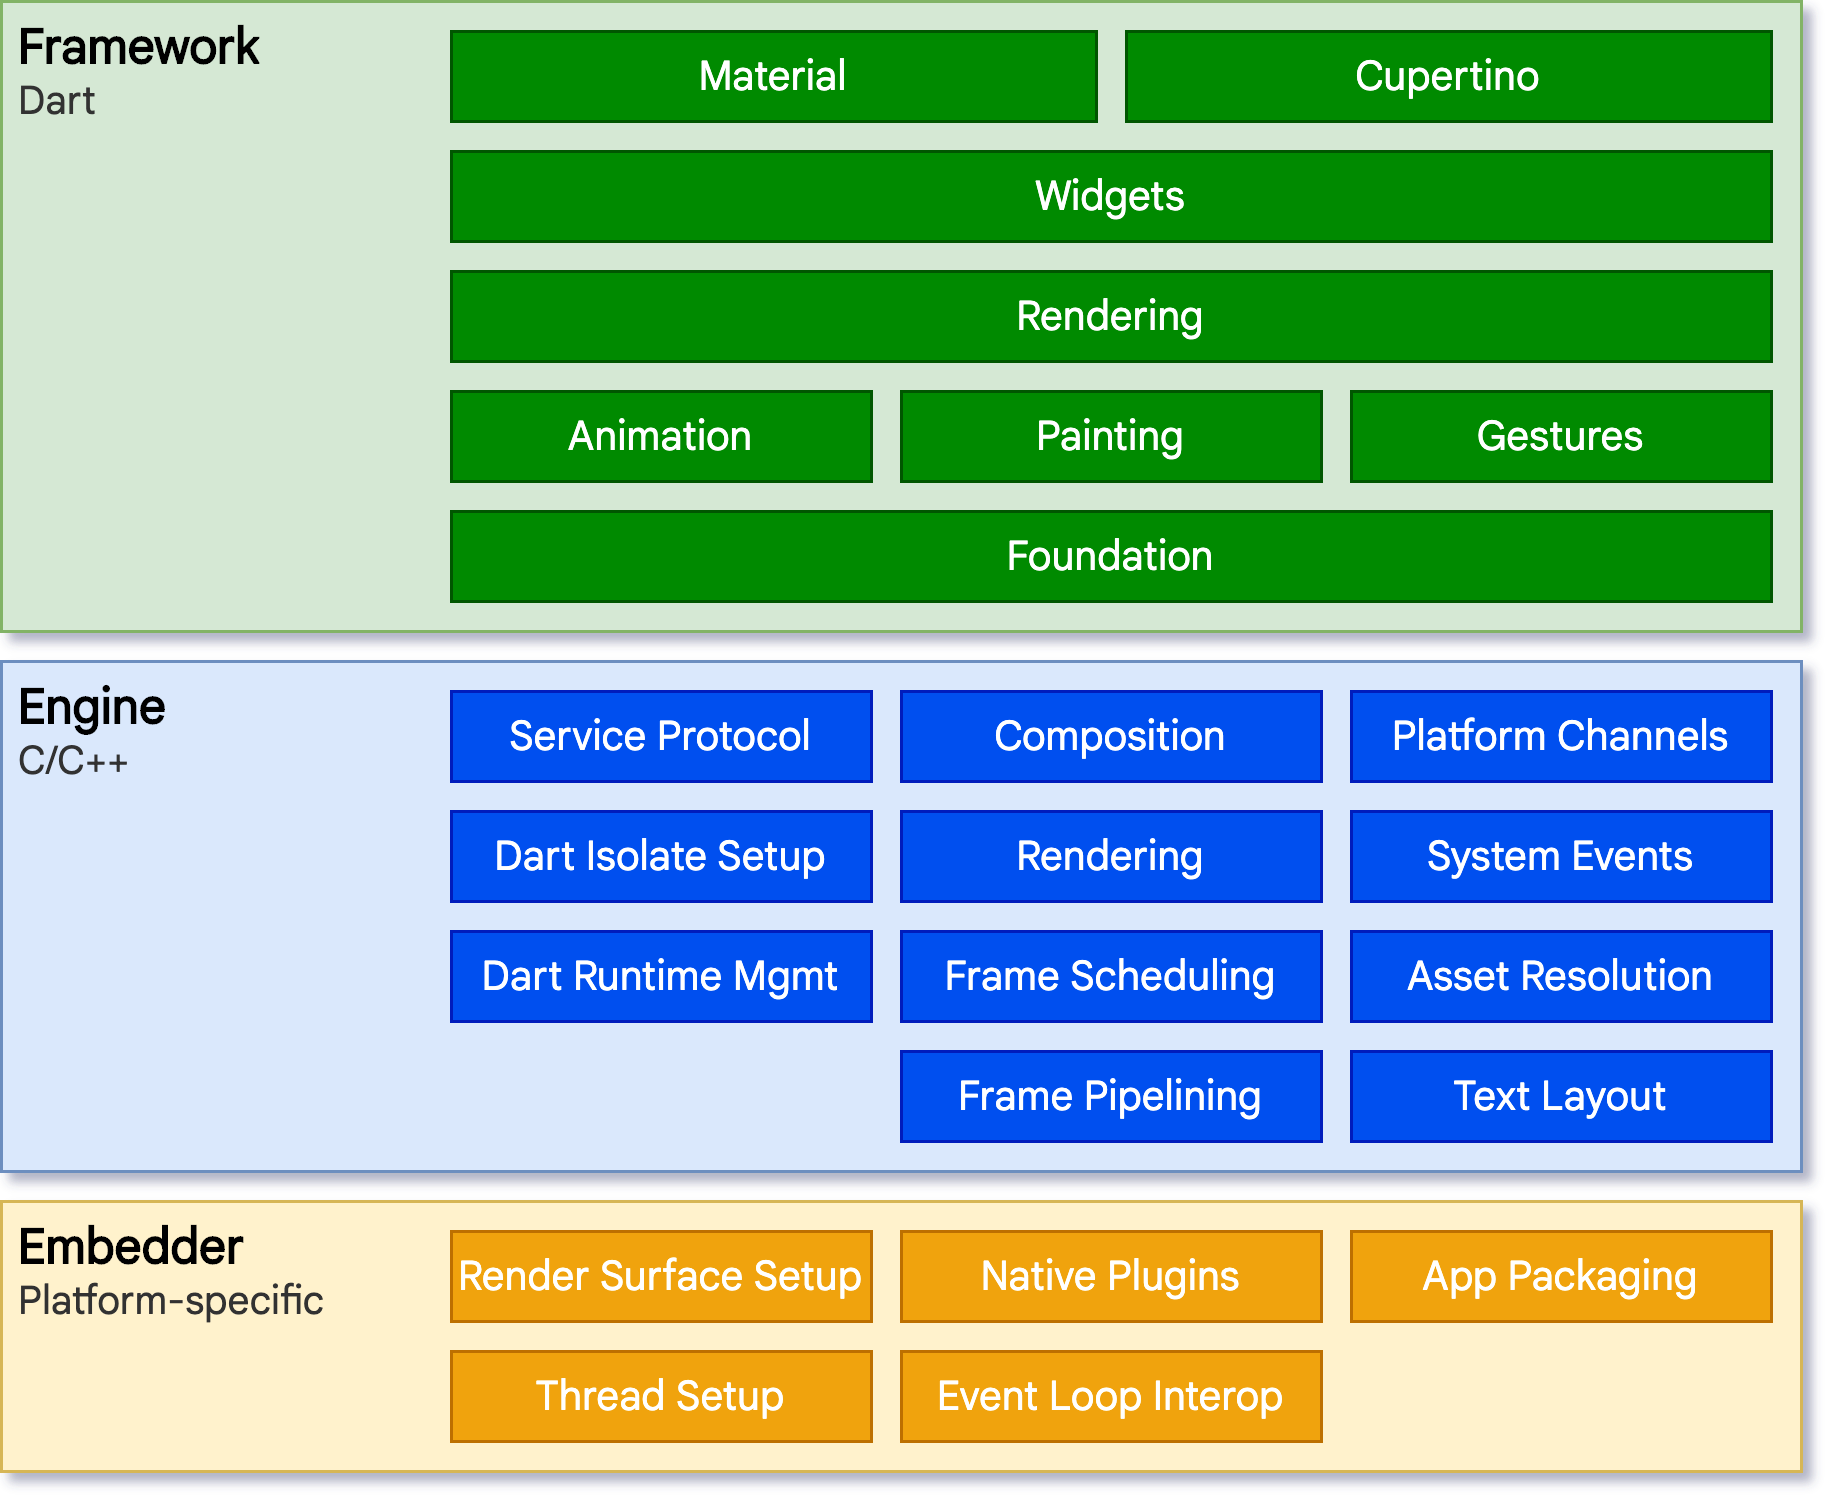
\includegraphics[width=0.9\linewidth]{img/architecture/mobile_clean_architecture.png}
    \caption{\textit{Kiến trúc Phân tầng Clean Architecture của Ứng dụng MyHCMUT}}
    \label{fig:mobile_clean}
\end{figure}

\begin{itemize}
    \item \textbf{Tầng Trình diễn (Presentation Layer):} Chứa các Pages, Widgets và Riverpod Notifiers. Tầng này chịu trách nhiệm hiển thị UI, lắng nghe tương tác người dùng và phản ánh trạng thái \texttt{AsyncValue} (loading, data, error).
    \item \textbf{Tầng Nghiệp vụ (Domain Layer):} Chứa các Entities, Freezed DTOs và quy tắc nghiệp vụ phía client (validation form, parsing dữ liệu).
    \item \textbf{Tầng Dữ liệu (Data Layer):} Chứa các Repositories, Data Sources, Network Client (Dio) và Local Cache (SQLite / Secure Storage). Tầng này chịu trách nhiệm điều phối dữ liệu từ bộ nhớ đệm cục bộ và gọi API từ xa.
\end{itemize}

\subsection{Thiết kế Hệ thống Giao diện Material 3 Semantic Tokens (\texttt{global\_system})}
Toàn bộ màu sắc, khoảng cách (spacing), kiểu chữ (typography) và thành phần giao diện (Cards, Badges, InputFields, Buttons) được chuẩn hóa thành gói \texttt{packages/core/global\_system}. Các màu sắc được định nghĩa theo ngữ nghĩa (Semantic Tokens: \texttt{primary}, \texttt{surface}, \texttt{statusPending}, \texttt{statusApproved}, \texttt{statusRejected}) giúp ứng dụng tự động tương thích hoàn hảo giữa hai chế độ giao diện Sáng (Light Mode) và Tối (Dark Mode).

\section{Thiết kế Tích hợp API và Thông báo Đẩy}
\label{sec:api_notification_design}

\subsection{Thiết kế Bộ điều phối Token Đa miền (\texttt{MultiDomainAuthInterceptor})}
Do ứng dụng di động kết nối đồng thời với 3 dịch vụ Backend độc lập có base URL khác nhau, nhóm thiết kế một Interceptor duy nhất tại \texttt{packages/core/network}:
\begin{itemize}
    \item Tự động trích xuất chuỗi JWT \texttt{token\_auth} từ \texttt{flutter\_secure\_storage}.
    \item Tự động gắn tiêu đề \texttt{Authorization: Bearer <token>} vào mọi request gửi ra ngoài.
    \item Lắng nghe phản hồi HTTP 401 Unauthorized: Nếu phát hiện Token hết hạn, Interceptor tự động kích hoạt luồng làm mới Token ngầm (Silent Refresh) và phát lại request gốc mà không làm gián đoạn trải nghiệm của người dùng.
\end{itemize}

\subsection{Thiết kế Dữ liệu Thông báo Đẩy có Cấu trúc (Structured Metadata)}
Để loại bỏ sự phụ thuộc vào việc bóc tách chuỗi URL web (\texttt{targetLink}) không ổn định, nhóm thiết kế cấu trúc payload thông báo chuẩn hóa từ Backend tới Mobile gồm 4 trường Metadata có cấu trúc:
\begin{itemize}
    \item \texttt{source}: Định danh phân hệ phát sinh thông báo (\texttt{'hrm'} hoặc \texttt{'ioffice'}).
    \item \texttt{entityType}: Loại đối tượng nghiệp vụ (\texttt{'leave'}, \texttt{'business-trip'}, \texttt{'incoming-doc'}, \texttt{'outgoing-doc'}, \texttt{'task'}).
    \item \texttt{entityId}: Khóa chính định danh bản ghi cụ thể (ví dụ ID đơn nghỉ phép hoặc ID nhiệm vụ).
    \item \texttt{isApproval}: Cờ đánh dấu màn hình duyệt dành cho cấp quản lý (\texttt{'true'} / \texttt{'false'}).
\end{itemize}

\noindent Khi người dùng nhấn vào thông báo trên điện thoại, lớp \texttt{NotificationRouteParser} phân tích trực tiếp 4 trường này để kích hoạt \texttt{GoRouter} điều hướng thẳng đến đúng màn hình chi tiết tương ứng (Deep Linking).
